% !TEX TS-program = pdflatex
% ATS-friendly, single-column CV based on UpdateCV_GDO.tex.
% Keep the exported PDF text-based; do not print/scan it before uploading.
\documentclass[10pt,a4paper]{article}

\usepackage[a4paper,margin=1.45cm]{geometry}
\usepackage[T1]{fontenc}
\usepackage[utf8]{inputenc}
\usepackage{lmodern}
\usepackage[english]{babel}
\usepackage{enumitem}
\usepackage{graphicx}
\usepackage{xcolor}
\usepackage[hidelinks,unicode]{hyperref}
\usepackage{titlesec}
\usepackage{parskip}
\usepackage{microtype}

\renewcommand{\familydefault}{\sfdefault}
\input{glyphtounicode}
\pdfgentounicode=1
\pagestyle{empty}
\setlength{\parindent}{0pt}
\setlength{\parskip}{2.5pt}
\setlist[itemize]{leftmargin=1.25em,itemsep=1pt,topsep=2pt,parsep=0pt,partopsep=0pt}

\definecolor{SectionBlue}{HTML}{0A5275}
\titleformat{\section}
  {\large\bfseries\color{SectionBlue}}
  {}{0pt}{}[\vspace{-2pt}\titlerule]
\titlespacing*{\section}{0pt}{8pt}{3pt}

% Simple text-only entries preserve a predictable top-to-bottom reading order.
\newcommand{\role}[4]{%
  \textbf{#1} --- \textbf{#2}\par
  #3 \enspace|\enspace #4\par
}

\newcommand{\project}[3]{%
  \textbf{#1} \enspace|\enspace #2\par
  #3\par
}

\begin{document}

% The portrait occupies only the header's right side; all ATS-relevant text stays
% in a single, uninterrupted text block and the remainder is one column.
\noindent
\begin{minipage}[c]{0.80\textwidth}
  {\LARGE\bfseries Grace Duquiza Olesen}\par
  \vspace{2pt}
  {\large Software Engineer }\par
  \vspace{4pt}
  Aarhus, Denmark \enspace|\enspace Full work authorization\par
  \href{mailto:duquizagrace03@gmail.com}{duquizagrace03@gmail.com} \enspace|\enspace +45 71 39 25 48\par
  \href{https://graceduquiza.github.io}{graceduquiza.github.io} \enspace|\enspace
  \href{https://www.linkedin.com/in/graceduquizaolesen}{linkedin.com/in/graceduquizaolesen}\par
  \href{https://github.com/graceduquiza}{github.com/graceduquiza}
\end{minipage}%
\hfill
\begin{minipage}[c]{0.16\textwidth}
  \raggedleft
  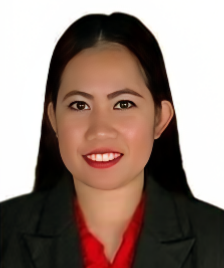
\includegraphics[width=2.7cm,height=3.2cm,keepaspectratio]{GDO.png}
\end{minipage}

\section{Professional Summary}
Software Engineer completing a BSc in Computer Science by October 2026 and available to start full-time employment. 
Hands-on experience building and deploying full-stack web and mobile applications, REST APIs, relational databases, 
authentication systems, and data-informed solutions. 
Python data analysis experience includes large-scale UK Biobank data and a peer-reviewed publication. 
Practical, persistent problem-solver with international experience and a strong focus on software quality and user needs.

\section{Technical Skills}
\textbf{Programming Languages:} Python, Java, C++, JavaScript, TypeScript, SQL\par
\textbf{Frontend:} React, Next.js, HTML, CSS, Tailwind CSS, responsive design\par
\textbf{Backend and APIs:} ASP.NET Core, Node.js, Express.js, REST APIs, JSON Web Tokens (JWT)\par
\textbf{Databases and Data Analysis:} PostgreSQL, Supabase, SQLite, Pandas, NumPy, SciPy, Matplotlib, Seaborn, Pearson correlation, regression\par
\textbf{Tools and Cloud:} Git, GitHub, Docker, Microsoft Azure, Vercel, Firebase, Capacitor\par
\textbf{Core Knowledge:} Object-oriented programming, data structures and algorithms, software engineering, database systems, web development, machine learning, systems analysis and design

\section{Relevant Experience}
\role{Data Analyst Intern (Remote)}{Nightingale Project, Johannes Gutenberg University Mainz}{April 2025--July 2025}{Denmark}
\begin{itemize}
  \item Analyzed large-scale UK Biobank health and environmental data using Python, Pandas, NumPy, SciPy, Pearson correlation, and regression.
  \item Created data visualizations with Matplotlib and Seaborn, documented analytical methods, and collaborated with an international research team.
  \item Co-authored a peer-reviewed publication: \href{https://doi.org/10.21698/rjeec.2025.210}{doi.org/10.21698/rjeec.2025.210}.
\end{itemize}

\role{Housekeeper (Part-Time)}{Scandic Hotels}{February 2024--Present}{Aarhus, Denmark}
\begin{itemize}
  \item Prepare guest rooms to Scandic standards for cleanliness, hygiene, and presentation; replenish amenities, report maintenance concerns, and collaborate with the housekeeping team.
\end{itemize}

\role{Customer-Facing Operations Roles}{Retail, Hospitality, and Cosmetics}{December 2009--October 2019}{Philippines and United Arab Emirates}
\begin{itemize}
  \item Progressed through Sales Assistant, Sales Advisor, Cashier, Front Desk Cashier, Sales Consultant, and Beauty Advisor roles.
  \item Supported customers, financial transactions, inventory, displays, and daily operations across multicultural workplaces.
\end{itemize}

\section{Software Projects}
\project{Nutri-Tsek --- BSc Thesis}{2026}{Next.js, TypeScript, ASP.NET Core, PostgreSQL, REST APIs, JWT, Android, Capacitor}
\begin{itemize}
  \item Built and deployed a full-stack web and Android application with REST APIs, authentication, barcode scanning, nutrition scoring, testing, cloud deployment, and ongoing maintenance.
  \item Live application: \href{https://nutritsek.duquizaolesen.com}{nutritsek.duquizaolesen.com}; source code: \href{https://github.com/GraceDuquiza/Nutri-Tsek}{github.com/GraceDuquiza/Nutri-Tsek}.
\end{itemize}

\project{Online Python Tutor --- Modernized Fork}{2025}{Python, JavaScript, open-source maintenance}
\begin{itemize}
  \item Modernized an existing codebase by replacing deprecated modules, removing exposed API keys, resolving warnings, and verifying Python 3.6--3.14 compatibility.
  \item Source code: \href{https://github.com/GraceDuquiza/OnlinePythonTutor-Py3}{github.com/GraceDuquiza/OnlinePythonTutor-Py3}.
\end{itemize}

\newpage
\section{Software Projects (continued)}
\project{Danish Vocabulary Trainer}{2025}{HTML, CSS, JavaScript}
\begin{itemize}
  \item Developed a mobile-friendly study and quiz application with bilingual vocabulary, grammar lessons, exercises, and answer keys.
  \item Live demo: \href{https://graceduquiza.github.io/Danish_Vocab_Trainer/}{graceduquiza.github.io/Danish\_Vocab\_Trainer}.
\end{itemize}

\project{Sudoku Learn}{2025}{JavaScript, responsive design, LocalStorage}
\begin{itemize}
  \item Created a learning-focused game with 4x4 and 9x9 boards, state management, smart hints, undo/redo, and automatic progress saving.
  \item Live demo: \href{https://graceduquiza.github.io/SudokuGame/}{graceduquiza.github.io/SudokuGame}.
\end{itemize}

\section{Education}
\role{Bachelor of Science in Computer Science}{AMA University Online Education}{2021--Expected graduation: October 2026}{Quezon City, Philippines (Online)}
Coursework: Software Engineering, Data Structures and Algorithms, Database Systems, Object-Oriented Programming, Web Development, Machine Learning, and Systems Analysis and Design.

\role{Accountancy Short Course}{Filipino Institute UAE}{2018}{Dubai, United Arab Emirates}
Completed the course with Third Honors in Accounting.

\role{Bachelor of Science in Accountancy}{Carlos Hilado Memorial State College}{2012--2013}{Bacolod City, Philippines}
Completed one year of the degree program.

\section{Professional Development}
\role{Mentee}{Danish Data Science Academy Mentorship Programme}{October 2025--June 2026}{Denmark}
Selected to develop data science, research, and career-planning skills through mentorship activities and networking with data science professionals.

\role{Danish Language --- Pr\o ve i Dansk 3 (PD3)}{AOF}{2024--2025}{Denmark}
Passed the Pr\o ve i Dansk 3 (PD3) examination.

\role{FVU Danish Language Studies}{CLAVIS}{2024--Present}{Denmark}
Continuing to develop Danish-language and workplace communication skills through FVU studies.

\section{Additional Experience}
\role{Au Pair --- Cultural Exchange}{Egersund, Norway}{November 2021--June 2023}{Norway}
Provided childcare and household support while strengthening responsibility, flexibility, and cross-cultural communication.

\role{Au Pair --- Cultural Exchange}{Risskov, Denmark}{November 2019--October 2021}{Denmark}
Provided household support while adapting to a new country, culture, and language.

\section{Languages and Additional Skills}
\textbf{Languages:} English (fluent), Danish (PD3 certified), Hiligaynon (mother tongue), Tagalog (native proficiency)\par
\textbf{Professional Skills:} Practical problem solving, continuous learning, persistence, responsibility, adaptability, and cross-cultural collaboration\par
\textbf{Honor:} Third Honor, Accounting, Filipino Institute UAE (2018)

\end{document}
